% =====================================================================
%  Short paper — PSP 8 — Universidade de Brasília
%  Para compilar no Overleaf: Menu > Compiler > pdfLaTeX
%  Coluna única, espaçamento simples (linespread 1.0)
% =====================================================================
\documentclass[10pt,a4paper]{article}

\usepackage[utf8]{inputenc}
\usepackage[T1]{fontenc}
\usepackage[brazil]{babel}
\usepackage[margin=2.8cm]{geometry}
\usepackage{times}
\usepackage{graphicx}
\usepackage{booktabs}
\usepackage{amsmath}
\usepackage{microtype}
\usepackage{url}
\usepackage[hidelinks]{hyperref}
\usepackage{caption}

\linespread{1.0}                       % espaçamento simples
\captionsetup{font=small,labelfont=bf,skip=4pt,width=0.85\textwidth}
\setlength{\parskip}{0pt}
\setlength{\columnsep}{0.7cm}
\renewcommand{\arraystretch}{1.05}
\usepackage{titlesec}
\titlespacing*{\section}{0pt}{1.4ex plus .2ex}{0.7ex}
\titlespacing*{\subsection}{0pt}{1.1ex plus .2ex}{0.5ex}
\titlespacing*{\paragraph}{0pt}{0.9ex plus .1ex}{1em}
\titleformat*{\section}{\large\bfseries}
\titleformat*{\subsection}{\normalsize\bfseries}
\setlength{\textfloatsep}{10pt plus 2pt minus 2pt}
\setlength{\intextsep}{10pt plus 2pt minus 2pt}
\setlength{\abovedisplayskip}{6pt}
\setlength{\belowdisplayskip}{6pt}
\usepackage{enumitem}
\setlist{nosep,leftmargin=*}

\title{\vspace{-1.2cm}\textbf{Da base bruta ao plano de retenção:\\
um pipeline de dados em nuvem e o custo metodológico\\
de comparações mal construídas}}

\author{
  Isadora Messenberg Guimarães Macêdo Rebello \\
  \small Matrícula 231013387 \\
  \small Departamento de Engenharia de Produção --- Universidade de Brasília \\
  \small Projeto de Sistema de Produção 8 --- Prof. André Luiz Marques Serrano
}
\date{\small Novembro de 2026}

\begin{document}
\maketitle

\begin{abstract}
\noindent
\small
Este trabalho constrói um pipeline de dados em nuvem que transforma o cadastro bruto de
7.043 clientes de uma operadora de telecomunicações em um plano de retenção priorizado e
persistido. O pipeline implementa arquitetura em três camadas sobre a plataforma
Databricks, com perfilamento de qualidade em seis dimensões, modelagem dimensional em
esquema estrela e catálogo de dados com domínios e linhagem. Sobre essa base, quatro
níveis de análise respondem a seis perguntas de negócio. A contribuição metodológica
está em três verificações habitualmente omitidas em trabalhos de previsão de
cancelamento: a calibração das probabilidades antes de convertê-las em valor monetário, a
escolha do ponto de corte por valor esperado em vez de métrica estatística simétrica, e a
checagem de suporte empírico dos contrafactuais usados na camada prescritiva. Os
resultados mostram que a vantagem da abordagem estatística sobre a regra de negócio é
sólida em ordenação de risco (\(\Delta\)AUC de \(+0{,}035\), IC 95\% \([+0{,}022;
+0{,}048]\), superior em 100\% de 25 reamostragens) mas incerta em resultado financeiro
(IC 95\% cruzando zero). Duas conclusões de uma versão anterior deste MVP não
sobreviveram ao reteste contra adversários tradicionais construídos na sua melhor versão:
a superioridade da clusterização em segmentação desapareceu, e o ganho prescritivo caiu
de \(+130\%\) para \(+53\%\). Uma das três ações prescritas revelou-se extrapolação, com
apenas 19\% dos clientes elegíveis em região de sobreposição empírica.

\vspace{4pt}
\noindent\textbf{Palavras-chave:} pipeline de dados; modelagem dimensional; qualidade de
dados; previsão de cancelamento; análise prescritiva; calibração.
\end{abstract}

% =====================================================================
\section{Introdução}

A retenção de clientes em telecomunicações é um problema de margem antes de ser um
problema de previsão. Adquirir um assinante custa múltiplos da mensalidade, de modo que
cada cancelamento evitado tem retorno direto. O obstáculo operacional é que a área
comercial costuma descobrir a intenção de cancelar no momento em que o cliente liga para
cancelar --- quando a retenção já é cara e pouco eficaz.

Este trabalho trata o problema como engenharia de dados, e não apenas como exercício de
modelagem. A hipótese testada é: \emph{a partir exclusivamente do cadastro e da fatura, é
possível operar um pipeline que entregue periodicamente ao time comercial uma lista
priorizada de clientes em risco, com a ação de retenção indicada para cada um e o retorno
esperado dessa ação.} O produto mínimo capaz de testar essa hipótese não é um modelo
preditivo isolado, mas o percurso completo: ingestão, perfilamento de qualidade,
modelagem dimensional, carga em repositório persistente e análise.

Seis perguntas de negócio orientam o trabalho: (P1) quanto da receita mensal está em
risco e onde se concentra; (P2) quais atributos explicam o cancelamento depois de
controlados os demais; (P3) se o cancelamento é previsível e se o ganho resiste a
amostras distintas; (P4) se as probabilidades estimadas são confiáveis o bastante para
sustentar contas em dinheiro; (P5) qual alocação de orçamento maximiza o retorno e qual o
ganho sobre uma regra de negócio bem construída; e (P6) se o modelo trata grupos
demográficos de forma equilibrada.

O trabalho parte de uma versão anterior do mesmo MVP, desenvolvida pela autora, que
comparava análise tradicional e aprendizado de máquina em cinco pares e concluía pela
superioridade da segunda em cinco de cinco indicadores. A revisão crítica dessa versão é
parte do objeto deste artigo. Três das verificações aqui introduzidas --- calibração,
critério de corte econômico e suporte do contrafactual --- alteram ou qualificam
conclusões anteriores, e o fazem na direção de reduzir, não ampliar, a vantagem atribuída
aos métodos estatísticos.

% =====================================================================
\section{Revisão}

\subsection{Arquitetura analítica de dados}

O esquema estrela de Kimball e Ross \cite{kimball} --- uma tabela fato cercada de dimensões
desnormalizadas --- permanece o padrão para cargas voltadas à consulta de negócio, ante a
alternativa normalizada de Inmon \cite{inmon}, que privilegia integridade sobre legibilidade.
A arquitetura em camadas progressivas, popularizada como \emph{medallion}, depende em
armazenamento de objetos de camadas transacionais como a de Armbrust et al. \cite{armbrust}.
Quanto a qualidade, Wang e Strong \cite{wang} estabeleceram que se trata de construto
multidimensional definido pela adequação ao uso, e Batini e Scannapieco \cite{batini}
sistematizaram as seis dimensões aqui empregadas.

\subsection{Previsão de cancelamento}

Neslin et al. \cite{neslin}, em competição com participação de múltiplas equipes sobre dados reais de
telecomunicações, documentaram que diferenças grandes de técnica produzem diferenças
modestas de acurácia, e que o retorno financeiro depende mais da estrutura da campanha
do que do algoritmo. Verbeke et al. \cite{verbeke} avançaram o argumento decisivo para este trabalho: os
modelos de cancelamento são rotineiramente selecionados por métricas estatísticas, o que
resulta em escolha subótima do ponto de vista do lucro, e propõem um critério de máximo
lucro esperado em substituição. A assimetria entre custo de falso negativo e de falso
positivo também é central em Provost e Fawcett \cite{provost}, cujo arcabouço de valor esperado fundamenta a
escolha de limiar adotada na Seção~\ref{sec:metodos}.

\subsection{Calibração e comparação de modelos}

Ordenação e correção de nível são propriedades distintas: um classificador pode discriminar
bem e ainda emitir probabilidades enviesadas. Niculescu-Mizil e Caruana \cite{niculescu}
mapearam a calibração de diferentes famílias de algoritmos, e Zadrozny e Elkan
\cite{zadrozny} introduziram a regressão isotônica como correção não paramétrica. Quando a
probabilidade é insumo de cálculo monetário, a calibração deixa de ser refinamento e passa a
ser pré-requisito. Para comparar abordagens sobre as mesmas instâncias, Dietterich
\cite{dietterich} recomenda o teste de McNemar, aqui empregado.

\subsection{Contrafactuais e equidade}

A camada prescritiva estima o efeito de intervenções alterando atributos de registros
existentes. King e Zeng \cite{king} demonstram que inferências contrafactuais realizadas longe
dos dados observados tornam-se dependentes do modelo e não dos dados, e propõem verificar se o
ponto pertence à envoltória convexa da amostra; o teste de sobreposição por escore de
propensão \cite{rosenbaum} operacionaliza esse diagnóstico. Para a auditoria de disparidade
entre grupos utiliza-se a igualdade de oportunidade de Hardt et al. \cite{hardt}.

% =====================================================================
\section{Métodos}
\label{sec:metodos}

\subsection{Dados e plataforma}

Utiliza-se a base \emph{Telco Customer Churn} (IBM Sample Data Sets, publicada no Kaggle
sob Database Contents License v1.0): 7.043 assinantes descritos por 20 atributos de
cadastro, serviços e faturamento, mais o indicador de cancelamento. O arquivo original é
um CSV de 970.457 bytes. A base não contém identificadores diretos; o código de cliente é
sintético, de modo que não se aplica tratamento adicional sob a Lei 13.709/2018.

O pipeline executa na plataforma Databricks sobre Apache Spark \cite{zaharia}, com tabelas Delta registradas no Unity
Catalog sob o esquema \texttt{workspace.churn\_mvp}. A persistência é verificável após o
encerramento da sessão: as tabelas permanecem consultáveis por SQL.

\subsection{Camadas e transformação}

A camada \textbf{bronze} ingere o arquivo sem conversão, com todos os atributos como texto,
acrescentando apenas marcação de linhagem. A decisão é deliberada: erro em regra de
transformação torna-se corrigível por reprocessamento, sem retorno à fonte.

A camada \textbf{silver} aplica nove regras numeradas, das quais três afetam a interpretação.
T1 converte o faturamento acumulado e atribui zero aos 11 vazios; a regra de consistência R3
demonstra que todos correspondem a clientes com zero meses de casa, para os quais zero é o
valor correto e não uma imputação. T4 colapsa o nível ``sem serviço de internet'' em ``não''
nos sete atributos de serviço agregado, por já estar a informação no atributo de tecnologia
de acesso. T8 deriva o desvio tarifário, para testar a hipótese de que reajuste recente
antecede cancelamento.

A camada \textbf{gold} implementa esquema estrela com grão de um cliente por retrato:
tabela fato com seis chaves estrangeiras e sete métricas, e seis dimensões
(cliente, demografia, contrato, pagamento, internet e telefonia). A dimensão de internet
é dimensão-lixo, agregando sete atributos de baixa cardinalidade cujas 129 combinações
efetivamente observadas substituem as 2.187 teoricamente possíveis. A carga é validada
por três asserções: preservação do número de linhas, unicidade do grão e ausência de
chave estrangeira órfã.

O catálogo de dados documenta 31 atributos com tipo, descrição, domínio esperado,
obrigatoriedade e linhagem, persistido como tabela consultável e aplicado também como
comentário nativo das colunas Delta.

\subsection{Protocolo analítico}

A divisão treino/teste (75/25, estratificada, semente fixa) antecede qualquer análise; regras,
cortes, modelos e limiares são construídos exclusivamente sobre o treino. Implementados com
scikit-learn \cite{pedregosa}, comparam-se três classificadores (regressão logística, floresta
aleatória e \emph{gradient boosting}) com uma regra de pontuação de risco de cinco fatores
derivada das tabelas cruzadas do treino --- o equivalente ao que um analista produz em planilha.

\paragraph{Calibração.} Mede-se o escore de Brier e o erro de calibração esperado (ECE),
definido como a média ponderada de \(|\bar{y}_k - \bar{p}_k|\) sobre \(k\) faixas de
probabilidade prevista. Aplica-se regressão isotônica com validação cruzada interna.

\paragraph{Critério de corte.} Em lugar de maximizar F1, o limiar é escolhido por lucro
esperado:
\begin{equation}
\small
L(\tau) = \!\!\sum_{i:\,\hat{p}_i \geq \tau}\!\! \big(y_i \cdot m_i \cdot s \cdot h\big)
          \;-\; c \cdot \big|\{i : \hat{p}_i \geq \tau\}\big|
\end{equation}
em que \(m_i\) é a mensalidade, \(s = 0{,}30\) a taxa de sucesso da abordagem,
\(h = 12\) meses de horizonte e \(c = \textrm{US\$}\,30\) o custo de contato. As
premissas são ilustrativas e servem à comparação entre abordagens, não como previsão de
receita.

\paragraph{Estabilidade.} O experimento completo --- construção de regra, treino, calibração
e escolha de limiares --- é repetido sobre 25 divisões independentes, reportando-se a
distribuição das diferenças em AUC, F1 e lucro.

\paragraph{Adversários justos.} Duas comparações da versão anterior são refeitas contra
versões fortes da abordagem tradicional. Em segmentação, acrescenta-se a tabela cruzada
de \emph{duas} variáveis (contrato \(\times\) tempo de casa) às faixas de variável única
originalmente usadas. Em prescrição, acrescenta-se uma regra de atribuição de ação por
perfil à oferta única originalmente usada.

\paragraph{Suporte do contrafactual.}
\label{sec:prescritiva}
Para cada ação, ajusta-se um modelo de propensão que distingue clientes no estado de
origem dos já presentes no estado de destino, excluindo o atributo manipulado \emph{e seus
derivados}. Reporta-se a AUC dessa separação e a fração de clientes de origem cujo escore
cai na faixa de sobreposição entre os dois grupos.

% =====================================================================
\section{Resultados}
\label{sec:resultados}

\subsection{Qualidade dos dados}

O perfilamento revelou completude integral exceto pelo faturamento acumulado (99,84\%, 11
vazios) e conformidade integral nos 21 atributos. A regra R4 identificou 59 registros (0,8\%)
em que o acumulado diverge mais de 20\% do produto entre meses de casa e mensalidade, com erro
mediano de 2\%. A leitura não é de erro de dado, mas de defasagem conceitual: a mensalidade
registra a tarifa vigente e não a média histórica, de modo que os dois atributos medem
momentos distintos. A regra R6 encontrou 22 linhas idênticas exceto pelo identificador ---
clientes distintos com perfil igual, mantidos na carga.

A limitação mais séria é estrutural: \textbf{a base não possui marcação temporal alguma}.
Isso impede validação temporal, protocolo correto para previsão de cancelamento, e obriga ao
uso de divisão aleatória. O desempenho reportado adiante mede capacidade de reconhecer padrões
em uma população, não de prever o futuro a partir do passado.

\subsection{P1 --- Concentração da receita em risco}

O cancelamento atinge 26,5\% dos clientes e 30,5\% da receita: US\$ 139.131 de US\$ 456.117
mensais. Quem cancela paga US\$ 74,44 contra US\$ 61,27 de quem permanece --- 21\% a mais. A
perda é seletiva e recai sobre o cliente de maior valor, elevando o teto do investimento
racional em retenção.

\subsection{P2 --- Atribuição de causa}

As duas leituras concordam que tempo de casa e modalidade contratual lideram, e divergem no
meio da tabela --- onde a análise univariada erra sistematicamente. A forma de pagamento cai da
4\textsuperscript{a} para a 12\textsuperscript{a} posição: o cheque eletrônico exibe a maior
taxa isolada (45,3\%), mas quem paga assim é majoritariamente cliente mensal de fibra
recém-chegado. Mensalidade e ticket médio caem nove posições cada, pelo mesmo mecanismo; em
sentido oposto, atributos de \emph{streaming} e múltiplas linhas sobem de 11 a 13 posições.
A hipótese T8 foi \textbf{rejeitada}: o desvio tarifário ocupa a 22\textsuperscript{a} posição
entre 23, com importância de 0,0004. O resultado negativo é registrado e o atributo mantido no
catálogo.

\subsection{P3 e P4 --- Previsão, calibração e estabilidade}

A Tabela~\ref{tab:predicao} apresenta o desempenho no conjunto de teste sob os dois
critérios de corte. O teste de McNemar rejeita a hipótese de equivalência entre regra e
modelo em todos os casos (\(p < 10^{-10}\)); para a regressão logística, o modelo acerta
sozinho 210 clientes contra 43 da regra.

\begin{table}[t]
\centering
\small
\caption{Desempenho no teste (1.761 clientes) sob dois critérios de corte.}
\label{tab:predicao}
\begin{tabular}{@{}llrrr@{}}
\toprule
\textbf{Abordagem} & \textbf{Corte} & \textbf{F1} & \textbf{AUC} & \textbf{Lucro} \\
\midrule
Regra tradicional & F1    & 0,602 & 0,811 & 78.197 \\
Regra tradicional & Lucro & 0,543 & 0,811 & 81.518 \\
Reg.\ logística   & F1    & 0,629 & 0,847 & 79.952 \\
Reg.\ logística   & Lucro & 0,599 & 0,847 & \textbf{85.159} \\
\bottomrule
\end{tabular}
\end{table}

\paragraph{Calibração (P4).} A suspeita inicial não se confirmou: o ECE situa-se em 0,0146 já
sem tratamento --- quando o modelo estima 30\%, o cancelamento observado fica entre 28,5\% e
31,5\% --- e a recalibração isotônica o reduz a 0,0116. As probabilidades são utilizáveis em
cálculo financeiro. O ponto metodológico permanece: a versão anterior as empregou em contas de
valor esperado \emph{sem verificação}. O resultado foi favorável, mas é a verificação que
converte suposição em premissa documentada.

\paragraph{Critério de corte.} O efeito é material (Figura~\ref{fig:limiar}): o limiar cai de
0,31 (F1) para 0,13 (lucro) e o resultado sobe de US\$ 79.952 para US\$ 85.159 ---
\textbf{US\$ 5.207 adicionais com o mesmo modelo e os mesmos dados}. O F1 cai de 0,629 para
0,599, o que é esperado e irrelevante quando o objetivo é lucro e não simetria entre erros.

\begin{figure}[t]
\centering
\begin{minipage}{0.49\textwidth}\centering
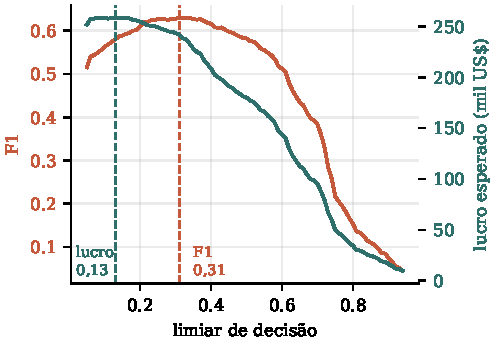
\includegraphics[width=\linewidth]{fig_limiar.pdf}
\end{minipage}\hfill
\begin{minipage}{0.49\textwidth}\centering
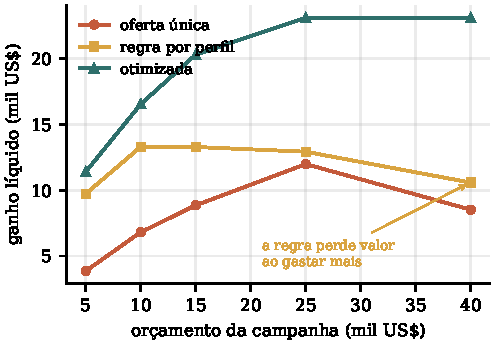
\includegraphics[width=\linewidth]{fig_sensibilidade.pdf}
\end{minipage}
\caption{\textbf{Esquerda:} os dois critérios de corte apontam limiares distintos --- maximizar
F1 leva a \(\tau = 0{,}31\), maximizar lucro esperado a \(\tau = 0{,}13\), com US\$ 5.207
adicionais no teste. \textbf{Direita:} sensibilidade ao orçamento --- a regra por perfil atinge
máximo em US\$ 10 mil e decresce por ordenar candidatos pelo risco e não pelo retorno, enquanto
o plano otimizado estabiliza ao esgotar os clientes de ganho esperado positivo.}
\label{fig:limiar}
\end{figure}

\paragraph{Estabilidade.} A Tabela~\ref{tab:estabilidade} mostra que a vantagem de
discriminação é sólida e a financeira não. Os intervalos de AUC e F1 não cruzam zero, com
superioridade em 100\% das 25 reamostragens. O do lucro cruza: em cerca de uma campanha a cada
25, a abordagem guiada por modelo renderia menos que a guiada por regra, porque o resultado
monetário depende de quais clientes caem na lista e de quanto pagam.

\begin{table}[t]
\centering
\small
\caption{Vantagem do modelo sobre a regra em 25 divisões independentes.}
\label{tab:estabilidade}
\begin{tabular}{@{}lrlr@{}}
\toprule
\textbf{Métrica} & \textbf{Média} & \textbf{IC 95\%} & \textbf{Vence} \\
\midrule
\(\Delta\) AUC   & $+0{,}035$ & $[+0{,}022;\,+0{,}048]$ & 100\% \\
\(\Delta\) F1    & $+0{,}058$ & $[+0{,}040;\,+0{,}074]$ & 100\% \\
\(\Delta\) Lucro & $+2.693$   & $[-952;\,+4.368]$       & 96\%  \\
\bottomrule
\end{tabular}
\end{table}

\subsection{Segmentação: o efeito do adversário}

A Tabela~\ref{tab:segmentacao} reporta o achado mais contundente do reteste. Uma tabela
cruzada de duas variáveis, construível em planilha, \textbf{supera o K-Means com 19
variáveis}. A silhueta de 0,134 confirma a ausência de agrupamentos naturais fortes: o
algoritmo particiona um espaço contínuo em vez de descobrir estrutura.

\begin{table}[t]
\centering
\small
\caption{Separação de risco entre segmentos, conjunto de teste.}
\label{tab:segmentacao}
\begin{tabular}{@{}lrr@{}}
\toprule
\textbf{Segmentação} & \textbf{Variáveis} & \textbf{Separação} \\
\midrule
Faixas de tempo de casa      & 1  & 0,1589 \\
K-Means (\(k=6\))            & 19 & 0,1949 \\
Contrato \(\times\) tempo    & 2  & \textbf{0,1969} \\
\bottomrule
\end{tabular}
\end{table}

A vantagem de 32\% atribuída à clusterização na versão anterior media a fraqueza do adversário,
não a força do método: isso não desqualifica a clusterização, qualifica a comparação. O segmento
crítico (mensal com menos de um ano, 52,4\% de cancelamento) é identificado pelas duas
abordagens, mas só a de negócio é explicável ao time comercial sem intermediação.

\subsection{P5 --- Prescrição e suporte do contrafactual}

O diagnóstico de sobreposição (Tabela~\ref{tab:suporte}) revelou que as três ações não são
igualmente confiáveis. A migração para débito automático é segura: clientes de cheque eletrônico
e de cartão automático são populações semelhantes no restante dos atributos. A oferta de suporte
técnico gratuito é \textbf{extrapolação quase completa}: quem possui suporte quase sempre possui
também segurança, backup e proteção, pois contrata o pacote inteiro. Ativá-lo isoladamente para
quem não tem nenhum agregado produz um perfil quase inexistente na base --- apenas 19\% dos
elegíveis têm contraparte comparável --- e o número gerado depende do modelo, não dos dados,
exatamente na acepção de King e Zeng \cite{king}.

\begin{table}[t]
\centering
\small
\caption{Suporte empírico dos contrafactuais prescritivos.}
\label{tab:suporte}
\begin{tabular}{@{}lrrl@{}}
\toprule
\textbf{Ação} & \textbf{AUC} & \textbf{Sobrep.} & \textbf{Confiança} \\
\midrule
Débito automático & 0,747 & 98,3\% & alta \\
Contrato anual    & 0,896 & 75,3\% & média \\
Suporte técnico   & 0,998 & 19,0\% & \textbf{baixa} \\
\bottomrule
\end{tabular}
\end{table}

Quanto ao desempenho dos planos (Tabela~\ref{tab:prescricao}), a otimização por valor
esperado supera a oferta única em 130\% e a regra por perfil em 53\%. A distância entre
esses dois percentuais quantifica o quanto uma comparação mal construída infla o
resultado atribuído ao método.

\begin{table}[t]
\centering
\small
\caption{Planos de retenção sob orçamento de US\$ 15.000.}
\label{tab:prescricao}
\begin{tabular}{@{}lrrr@{}}
\toprule
\textbf{Plano} & \textbf{Client.} & \textbf{Ganho} & \textbf{ROI} \\
\midrule
Oferta única      & 250 & 8.851  & 59\%  \\
Regra por perfil  & 646 & 13.290 & 89\%  \\
Otimizada         & 452 & \textbf{20.318} & \textbf{135\%} \\
\bottomrule
\end{tabular}
\end{table}

A análise de sensibilidade (Figura~\ref{fig:limiar}, direita) revelou comportamento não
antecipado: \textbf{os dois planos tradicionais destroem valor quando o orçamento cresce}. A
regra por perfil rende US\$ 13.300 com US\$ 10.000 e apenas US\$ 10.579 com US\$ 40.000;
ambas ordenam por risco e não por retorno, e carecem de critério de parada --- seguem gastando
em clientes cujo ganho esperado é negativo. O plano otimizado estabiliza em US\$ 23.131 porque
interrompe a alocação quando o valor esperado se anula. Saber quando não agir é parte do valor
da abordagem, e não aparece em nenhuma métrica de classificação.


\subsection{P6 --- Equidade}

O gênero não produz efeito mensurável (\(\Delta\)recall de 0,009), o que recomenda removê-lo:
atributo sem poder preditivo e com potencial discriminatório apenas acrescenta risco. Duas
disparidades merecem registro. Clientes idosos são sinalizados a 80,4\% contra 50,0\% dos
demais; parte é legítima, pois seu cancelamento real é de 42,7\% contra 23,4\%, mas a AUC cai
para 0,798 contra 0,847 --- o modelo \emph{ordena pior} justamente o grupo que mais aborda.
Clientes com dependentes apresentam a maior disparidade de \emph{recall} (0,143): o modelo
captura 94,7\% dos cancelamentos entre quem não tem dependentes e 80,5\% entre quem tem.

% =====================================================================
\section{Conclusão}

O pipeline cumpre a hipótese do MVP: a partir do cadastro e da fatura, entrega 452 clientes
priorizados, com ação indicada, ganho esperado e nível de confiança da simulação, persistidos em
tabela Delta e em arquivo operacional. O percurso --- ingestão fiel, perfilamento em seis
dimensões, modelagem em estrela com catálogo e carga validada por asserção --- é reprodutível e
verificável após o encerramento da sessão.

A contribuição principal, contudo, é metodológica e tem sinal negativo. Três verificações
habitualmente omitidas alteraram materialmente as conclusões. A escolha do limiar por
valor esperado, em vez de F1, adicionou US\$ 5.207 sem qualquer mudança de modelo ou de
dado, confirmando em escala reduzida o argumento de Verbeke et al. \cite{verbeke}. A checagem de
sobreposição revelou que uma das três ações prescritas carece de suporte empírico,
produzindo números que dependem do modelo e não dos dados. E a reconstrução dos
adversários tradicionais na sua melhor versão eliminou a vantagem da clusterização em
segmentação e reduziu o ganho prescritivo de 130\% para 53\%.

Essa última constatação é a mais transferível. Comparações entre abordagem tradicional e
métodos estatísticos são frequentemente montadas com a primeira em versão deliberadamente
simplificada --- faixas de uma variável contra clusterização multivariada, oferta única
contra otimização individualizada. O resultado mede a fraqueza do adversário escolhido,
não a força do método proposto. Quando o adversário é construído com o cuidado que um
analista de fato empregaria, a vantagem sobrevive, mas com menos da metade da magnitude.

A separação entre superioridade estatística e superioridade financeira aponta no mesmo
sentido. O modelo ordena risco melhor de forma consistente e reprodutível; que isso
produza mais lucro em qualquer trimestre específico não se sustenta nos dados. A promessa
defensável é a primeira.

As limitações condicionam o alcance das conclusões. A ausência de marcação temporal impede
validação temporal e análise de sobrevivência; a base não contém dados comportamentais ---
chamados, reclamações, qualidade de sinal --- que são precisamente os sinais que antecedem o
cancelamento; e a camada prescritiva estima associação, não causa. A extensão prioritária é, por
isso, experimental e não algorítmica: um teste controlado é a única forma de validar os
US\$ 20.318 estimados. Seguem-na a ingestão incremental com carimbo de tempo, modelos de
\emph{uplift} e monitoramento de deriva sobre a tabela de qualidade já produzida pelo pipeline.

% =====================================================================
\begin{thebibliography}{99}
\footnotesize\setlength{\itemsep}{0pt}
\bibitem{batini} BATINI, C.; SCANNAPIECO, M. \emph{Data Quality: Concepts, Methodologies and Techniques}. Berlin: Springer, 2006.
\bibitem{armbrust} ARMBRUST, M. et al. Delta Lake: high-performance ACID table storage over cloud object stores. \emph{Proceedings of the VLDB Endowment}, v. 13, n. 12, p. 3411--3424, 2020.
\bibitem{dietterich} DIETTERICH, T. G. Approximate statistical tests for comparing supervised classification learning algorithms. \emph{Neural Computation}, v. 10, n. 7, p. 1895--1923, 1998.
\bibitem{hardt} HARDT, M.; PRICE, E.; SREBRO, N. Equality of opportunity in supervised learning. In: \emph{Advances in Neural Information Processing Systems} 29, 2016, p. 3315--3323.
\bibitem{inmon} INMON, W. H. \emph{Building the Data Warehouse}. 4. ed. Indianapolis: Wiley, 2005.
\bibitem{kimball} KIMBALL, R.; ROSS, M. \emph{The Data Warehouse Toolkit: The Definitive Guide to Dimensional Modeling}. 3. ed. Indianapolis: Wiley, 2013.
\bibitem{king} KING, G.; ZENG, L. The dangers of extreme counterfactuals. \emph{Political Analysis}, v. 14, n. 2, p. 131--159, 2006.
\bibitem{neslin} NESLIN, S. A. et al. Defection detection: measuring and understanding the predictive accuracy of customer churn models. \emph{Journal of Marketing Research}, v. 43, n. 2, p. 204--211, 2006.
\bibitem{niculescu} NICULESCU-MIZIL, A.; CARUANA, R. Predicting good probabilities with supervised learning. In: \emph{Proceedings of the 22nd International Conference on Machine Learning}, 2005, p. 625--632.
\bibitem{pedregosa} PEDREGOSA, F. et al. Scikit-learn: machine learning in Python. \emph{Journal of Machine Learning Research}, v. 12, p. 2825--2830, 2011.
\bibitem{provost} PROVOST, F.; FAWCETT, T. \emph{Data Science for Business}. Sebastopol: O'Reilly Media, 2013.
\bibitem{rosenbaum} ROSENBAUM, P. R.; RUBIN, D. B. The central role of the propensity score in observational studies for causal effects. \emph{Biometrika}, v. 70, n. 1, p. 41--55, 1983.
\bibitem{verbeke} VERBEKE, W. et al. New insights into churn prediction in the telecommunication sector: a profit driven data mining approach. \emph{European Journal of Operational Research}, v. 218, n. 1, p. 211--229, 2012.
\bibitem{wang} WANG, R. Y.; STRONG, D. M. Beyond accuracy: what data quality means to data consumers. \emph{Journal of Management Information Systems}, v. 12, n. 4, p. 5--33, 1996.
\bibitem{zadrozny} ZADROZNY, B.; ELKAN, C. Transforming classifier scores into accurate multiclass probability estimates. In: \emph{Proceedings of the 8th ACM SIGKDD}, 2002, p. 694--699.
\bibitem{zaharia} ZAHARIA, M. et al. Apache Spark: a unified engine for big data processing. \emph{Communications of the ACM}, v. 59, n. 11, p. 56--65, 2016.
\end{thebibliography}

\vspace{4pt}
\noindent\rule{\textwidth}{0.4pt}\\
\footnotesize
\textbf{Disponibilidade.} Código, notebook, catálogo de dados e evidências de execução
estão no repositório público do projeto. A base é obtida em
\url{https://www.kaggle.com/datasets/blastchar/telco-customer-churn}.

\end{document}
